\section{Change client}In this dialog you can change the settings of a client. There are the edit lines you may allready know from the "Add a new client" dialog and three extra rows. These rows are used to select what should happen with the entered values.\\
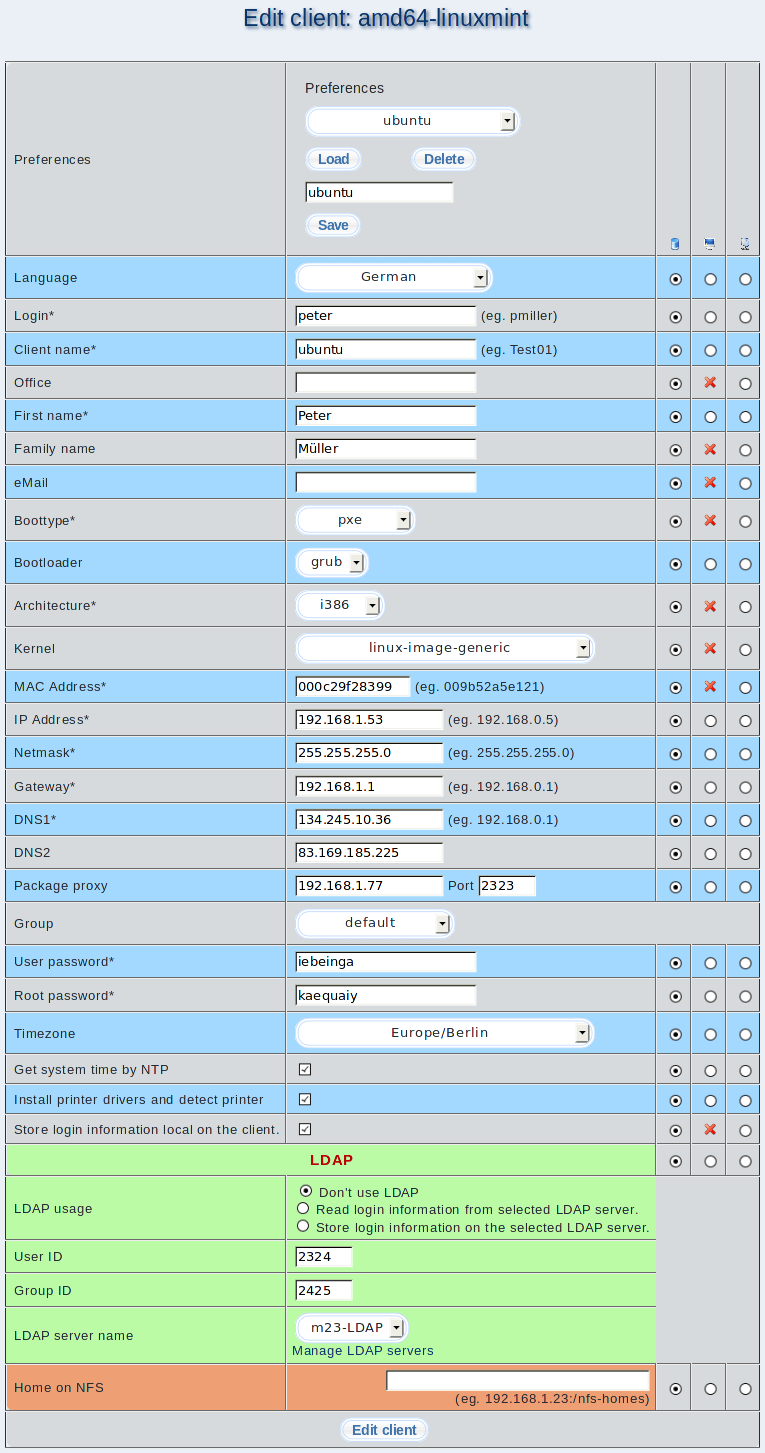
\includegraphics[scale=0.4]{/mdk/doc/manual/screenshots/en/edit_client.png} \\
\begin{itemize}
\item \textbf{Left row}: Select this row if you want to keep the value that is stored on the client and/or the server.\\
\item \textbf{Middle row}: The changes should be made on the client and transferred to the server afterwards.\\
\item \textbf{Right row}: The value is only written to the database on the server. This is useful if you made changes on client side by hand.\\
\end{itemize}
\subsection{Hint}
Some settings are only stored on the server. That's why these settings can't be made on the client. You can't select the middle row on those settings.\\
